\section{Experiments and Results}
We have ran all these models and experimented with them as we explored our data. In this section we will introduce these experiments and the significant results.

\subsection{Bag of Words - Term Frequency}
We applied the bag of words model to the different games' data-sets and got the frequency of word appearance in each. It is no surprise that for each game, the most frequent word was the game's name.

We wanted to compare the usage of offensive and Trump-related words and therefore we constructed Figure \ref{fig:bow-statistics}, it can be seen that \emph{Fifa} used the most racist inclined language, by a notable amount, and talked the most about Trump. We could also deduce from the figure that the games \emph{Dota2} and \emph{League of Legends} will probably have a low score in NEM for Trump-hate as they scarcely mention Trump.

It is also noticeable that one of the communities that used the most sexist words is \emph{The Sims}, which we were surprised at, since the target audience of \emph{The Sims} is comprised mostly of women. 

\begin{figure}[h]
    \begin{center}
        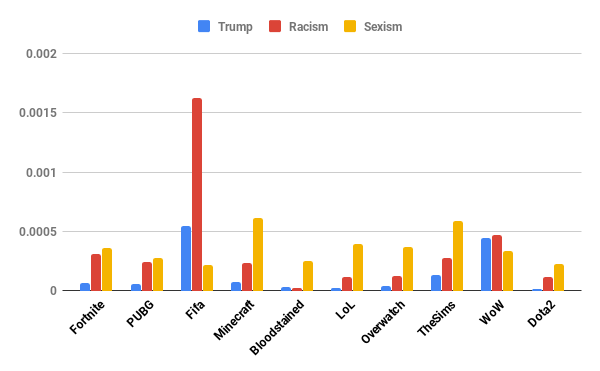
\includegraphics[scale=0.33]{Images/bow-statistics.png}
    \end{center}
    \caption{Percentage of sexist, racist and Trump related words in each game's community}
    \label{fig:bow-statistics}
\end{figure}


\subsection{Sentiment Analysis}
After applying the TextBlob sentiment analysis model to all posts we calculated the percentage of positive, neutral, and negative posts as shown in Figure~\ref{fig:Polarity}. It can be seen that in most communities the majority of posts are emotional as they are either positive or negative. We can also see clearly that the \emph{Bloodstained} community is far more negative which make sense as it is a violent game. On the opposite side, \emph{Word of Warcraft (WoW)} and \emph{League of Legends (LoL)} are very positive. In addition, \emph{Minecraft}, which is not a competitive game is fairly neutral.

\begin{figure}[h]
    \begin{center}
        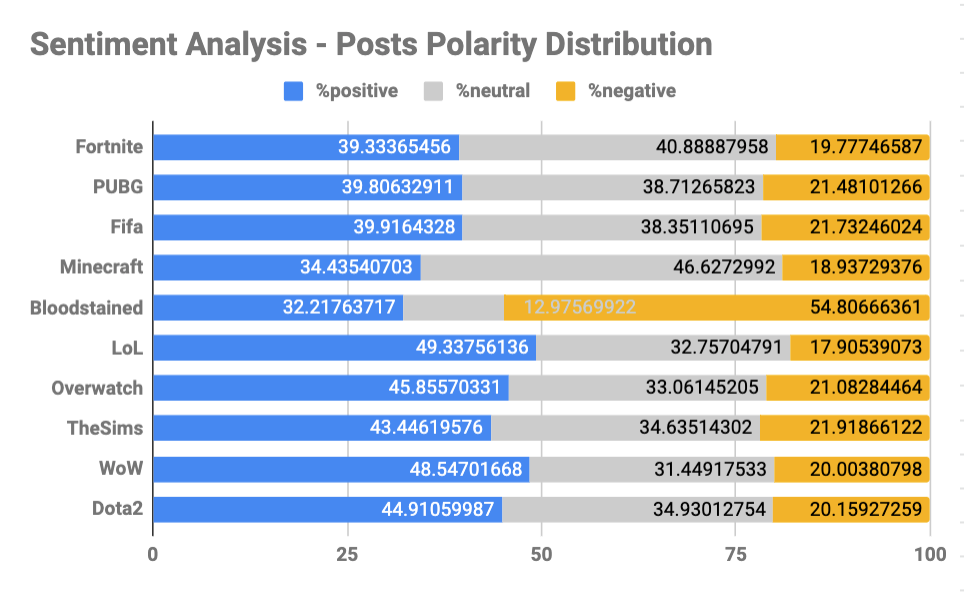
\includegraphics[scale=0.43]{Images/sentiment-analysis-polarity.png}
    \end{center}
    \caption{Blue bars represents percentage of Positive posts per game community, grey for Neutral and yellow for Negative sentiment.}
    \label{fig:Polarity}
\end{figure}

We also wanted to know, when taken to the extremes, how strong are the posts from each polarity, so we calculated the average for positive and negative polarity in every community as shown in Figure~\ref{fig:PolarityAverage}. We can see that \emph{Minecraft} players are more positive in their posted content and \emph{Bloodstained} as we seen before, are expressing stronger negative emotions.

\begin{figure}[h]
    \begin{center}
        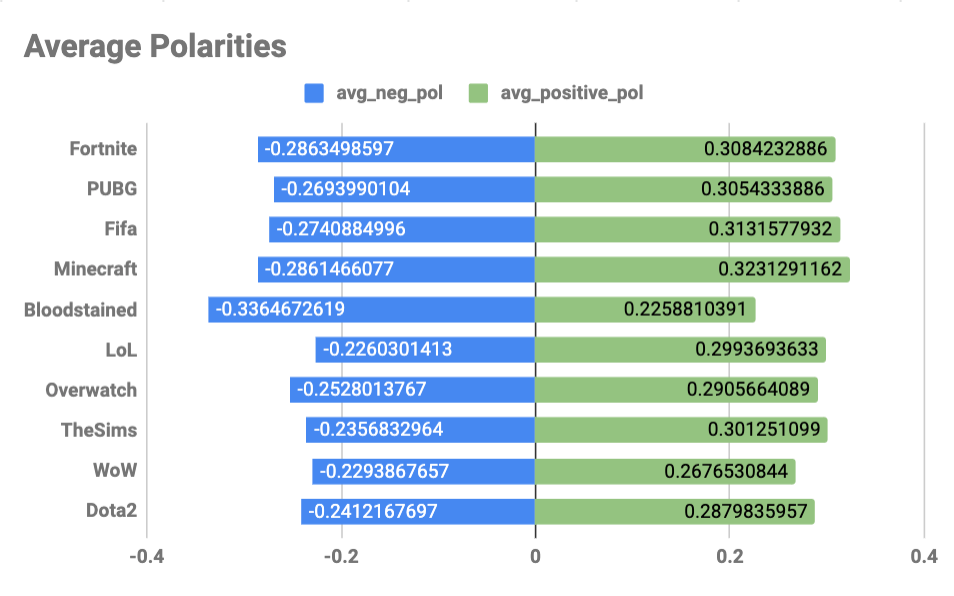
\includegraphics[scale=0.43]{Images/avg_polarities.png}
    \end{center}
    \caption{Blue bars represents the avg. value of all the negative polarity posts for that community while the green is avg of all positive polarity posts.}
    \label{fig:PolarityAverage}
\end{figure}


\subsection{Word Embedding}
We trained word embedding models for every game, evaluated their correctness and performed an iterative process of hyper-parameters tuning and retraining until we got embedding models that exhibit the essence of the gaming language.
Once achieved, we wanted to perform word triplets calculation and also extract the most similar words to each word in our groups of \emph{Neutral Words}. We will review some our interesting findings below.
\vspace{2mm}

When referring to women gamers in the game \emph{Fortnite} we got these triplets $Man\rightarrow Woman$ like $Gamer \rightarrow [\textbf{gamergirls}, egirl, greatgame]$ while when performing this on \emph{Fifa} we got $Man\rightarrow Woman$ like $Gamer \rightarrow [\textbf{meaningless}, exclude, prize]$ that show a much more discriminating attitude towards female players. 
\vspace{2mm}

When reviewing the different communities' politic affiliation, for the game \emph{Fortnite} we got that $Trump \rightarrow Muslim$ like $Man \rightarrow [\textbf{islamophobic}, huzzah, recruits]$ and that the most similar words to $Trump$ are $[toddler, donald, rat, president, tik, harass]$ while in the game \emph{PUBG} the triplet $Trump \rightarrow Clinton$ like $Man \rightarrow [\textbf{dumbest}, mess, alves]$ and the most similar words to $Trump$ are $[donald, cringe, iran, nonsense, act]$ these can indicate that \emph{PUBG} players are more right-winged than \emph{Fortnite} players that present a more liberal line.
\vspace{2mm}

When reviewing similar words in \emph{Fifa} the most similar words to $Arab$ are $[slave, gulf, \textbf{exploitation}, \textbf{immigrants}, qatar]$ and most similar words to $\textbf{Africans}$ are $[slaves, insult, slave, labor, \textbf{nigga}]$ which can indicate to a culture of racism.



\subsection{Negativity Evaluation Metric}
We calculated the different NEM metrics for $Sexsim, Racism, Trump-Hate$ in each game. While doing so, we experimented with the terms coefficients ($\alpha, \beta, \gamma$) and conclude to yield good results from the followings:

\begin{itemize}
\itemsep0em 
    \item $\gamma=0.6$ - the coefficient for the word embedding term, which we believe holds the most valuable contribution to our metric, hence we decided to grant it with the highest portion.
    \item $\alpha=0.3$ - the coefficient for the term frequency, which from our experimentation holds insight to community's linguistic choices, and therefore, is the second most important. 
    \item $\beta=-0.1$ - the coefficient for the sentiment, when experimenting with the results from the sentiment analysis model we found it to be inaccurate in some cases which puts it reliability in question so we decided to set it as the lowest contributing part. it has a negative value as the polarity score is negative.
\end{itemize}

When viewing the results of NEM Racism in Figure \ref{fig:nem-racism}, and as expected from the term frequency results, we can see that \emph{Fifa} is the most racist community with a score of 0.0472. It is worth mentioning that is not very high considering the values of NEM are [0,1].


Over-viewing all of the NEM values, Sexism got the highest scores with the game \emph{Dota2} scoring 0.0577.
The least sexist community as shown in Figure \ref{fig:nem-sexism} is \emph{The Sims} even though it had the highest score in the term frequency results. 

At first, Trump-hate in \emph{BloodStained} was unexpectedly high with a score of 0.02, however after further consideration, we have found this to be the result of one of our \emph{Neutral Words} for Trump being 'president', which seems to be related to the game, rather than the USA president. Furthermore, elimination of this word in this particular game resulted in score 0 for the Trump-hate metric.

In Figure \ref{fig:nem-trump2} we can see that even though \emph{Fortnite} got the highest score for NEM Trump-hate, it has a very low value of 0.007 which means the gaming communities scarcely mention Trump hence, do not engage in Trump-hate speech.

\begin{figure}[h]
    \begin{center}
        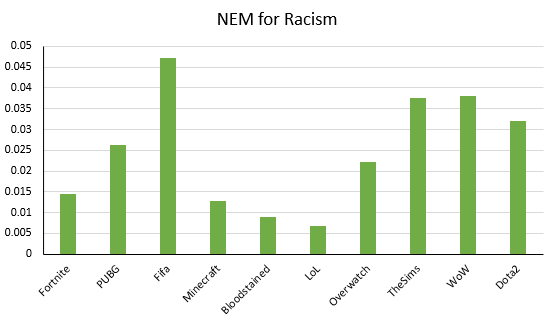
\includegraphics[scale=0.46]{Images/nem-racism-g.PNG}
    \end{center}
    \caption{NEM values for Racism property per game community}
    \label{fig:nem-racism}
\end{figure}

\begin{figure}[h]
    \begin{center}
        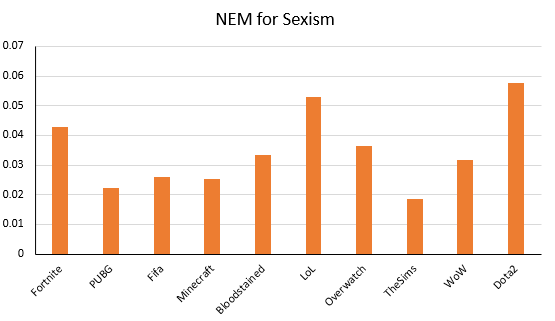
\includegraphics[scale=0.46]{Images/nem-sexism-r.PNG}
    \end{center}
    \caption{NEM values for Sexism property per game community}
    \label{fig:nem-sexism}
\end{figure}

\begin{figure}[ht]
    \begin{center}
        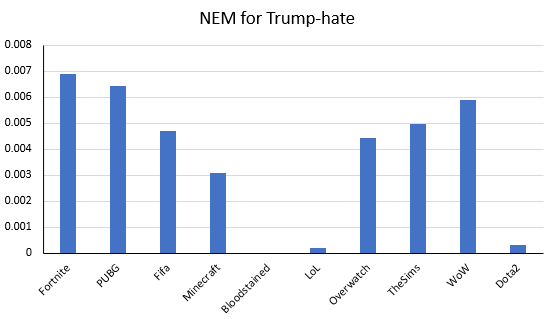
\includegraphics[scale=0.46]{Images/nem-trump2.PNG}
    \end{center}
    \caption{NEM values for Trump-hate property per game community after re-running NEM on Bloodstained without the word president}
    \label{fig:nem-trump2}
\end{figure}